% para complilar hacer
% pdflatex -jobname=Informe main.tex

\documentclass[12pt]{article}

% --- Paquetes Básicos ---
\usepackage[utf8]{inputenc}
\usepackage[spanish]{babel}
\usepackage{geometry}
\geometry{a4paper, margin=2.5cm}
\usepackage{amsmath, amsfonts} % Para fórmulas matemáticas si las necesitas
\usepackage{hyperref} % Para enlaces
\usepackage{graphicx} % Para insertar imágenes
\usepackage{float}    % Para usar el modificador [H] que fija la imagen en un lugar

% --- Datos del Informe ---
\title{Evolución de la Educación Superior en Bolivia: Un Estudio Temporal sobre el Crecimiento y la Desigualdad de Género en Matrículas y Titulaciones}
\author{Dávalos Alarcón Rodrigo \\
        Mamani Cahuana Daniel Edgar \\
        Flores Ulo Wilmer Alejandro \\
        Salinas Condori Ian Ezequiel \\
       }
\date{\today}
\begin{document}

\maketitle

\section*{Introducción}

En el contexto global y particularmente en Bolivia, las universidades han asumido el reto de reducir la desigualdad, buscando democratizar el acceso al crecimiento profesional. Sin embargo, este incremento en la oferta educativa ha generado una paradoja: en lugar de equilibrar la balanza, ha consolidado la capacidad técnica de los centros donde se originaron estos modelos (como Europa), dejando rezagadas a otras regiones.

Bolivia, como nación latinoamericana, enfrenta esta brecha con un agravante estructural: el predominio del comercio informal sobre el empleo formal. Esta realidad subraya la importancia crítica de la educación superior; no solo se trata de masificar la matrícula, sino de garantizar que la formación académica permita al país competir en estándares internacionales a largo plazo.

El presente informe analiza los datos históricos de las universidades en Bolivia para diagnosticar el panorama educativo actual y evaluar si el camino trazado es el adecuado para los desafíos futuros. Si bien el mercado laboral presenta dificultades evidentes para los nuevos profesionales, este estudio no se centra en la empleabilidad, sino en el comportamiento de la accesibilidad a la educación visto desde perspectiva de las matrículas. Se parte de la premisa de que la educación superior mantiene su vigencia y utilidad, incluso en sectores tradicionalmente informales como los negocios. Por tanto, esta investigación se limita a un análisis descriptivo y prospectivo de los datos académicos disponibles.

\section*{Objetivos}

\subsection*{Objetivo General}
Analizar la evolución temporal del crecimiento y las desigualdades de género en las matrículas y titulaciones de la educación superior en Bolivia, para identificar las áreas de estudio y ciudades con mayores brechas educativas.

\subsection*{Objetivos Específicos}

\begin{itemize}
    \item \textbf{Cuantificar la evolución de la matrícula:} Identificar las tasas de crecimiento anual de inscritos en el sistema universitario boliviano durante el periodo de estudio.
    \item \textbf{Identificar brechas de género:} Comparar la distribución de hombres y mujeres en las distintas áreas del conocimiento y niveles de titulación.
    \item \textbf{Analizar la concentración geográfica:} Determinar qué departamentos o ciudades concentran la mayor oferta y demanda académica, contrastándola con las zonas de menor acceso.
    \item \textbf{Evaluar la relación entre oferta y formalidad:} Explorar descriptivamente si las áreas de estudio con mayor crecimiento coinciden con los sectores económicos de mayor informalidad en el país.
    \item \textbf{Proyectar tendencias futuras:} Aplicar modelos descriptivos para estimar el comportamiento de la matrícula en los próximos años basándose en los datos históricos.
\end{itemize}

\section*{Metodología}

Para el análisis de los datos se usará lo que es la metodologia CRISP-DM que es un acrónimo de de Cross-Industry Standard Process for Data Mining. Este es un modelo de proceso estándar, ampliamente reconocido y utilizado en la industria, que describe los pasos necesarios para llevar a cabo con éxito un proyecto de minería de datos o de análisis de datos.

Este marco de trabajo proporciona una estructura iterativa y cíclica que organiza el flujo de trabajo en seis fases interconectadas, las cuales son:

\begin{enumerate}
  \item \textbf{Comprensión del Negocio (Business Understanding)}: Esta fase inicial se centra en la definición de los objetivos del proyecto y los requisitos desde una perspectiva de negocio. Se busca transformar este conocimiento en una definición de problema técnico y en un plan preliminar diseñado para alcanzar los objetivos establecidos.
  \item \textbf{Comprensión de los Datos (Data Understanding)}: Consiste en la recolección inicial de datos y la realización de actividades destinadas a familiarizarse con ellos. El propósito es identificar problemas de calidad, descubrir conocimientos preliminares o detectar subconjuntos interesantes de información para formar hipótesis sobre datos ocultos.
  \item \textbf{Preparación de los Datos (Data Preparation)}: Esta etapa abarca todas las actividades necesarias para construir el conjunto de datos final que será introducido en las herramientas de modelado. Las tareas incluyen la selección de tablas, registros y atributos, así como la limpieza y transformación de los datos para adecuarlos al análisis.
  \item \textbf{Modelado (Modeling)}: En esta fase se seleccionan y aplican diversas técnicas de modelado y se calibran sus parámetros a valores óptimos. Debido a que algunas técnicas requieren formatos de datos específicos, a menudo es necesario regresar a la fase de preparación de datos durante este proceso.
  \item \textbf{Evaluación (Evaluation)}: Una vez construido el modelo (o modelos), se debe evaluar su calidad y eficacia antes de proceder al despliegue. Se verifica si el modelo cumple con los objetivos de negocio definidos en la primera fase y se determina si existe alguna razón importante por la cual el modelo no deba ser utilizado.
  \item \textbf{Despliegue (Deployment)}: La creación del modelo no marca el final del proyecto. Los conocimientos obtenidos deben ser organizados y presentados de manera que el usuario final pueda utilizarlos. Dependiendo de los requisitos, esta fase puede ser tan simple como la generación de un informe o tan compleja como la implementación de un proceso de minería de datos repetible en la infraestructura de la organización.
\end{enumerate}

Las características principales de esta metodologia son que:

\begin{itemize}
  \item \textbf{Iteratividad}: El proceso no es estrictamente lineal. Es habitual retroceder a fases anteriores según los hallazgos realizados en etapas posteriores.
  \item \textbf{Neutralidad}: Es un estándar independiente de las herramientas tecnológicas o del sector industrial donde se aplique.
  \item \textbf{Orientación} a Objetivos: Prioriza los resultados de negocio sobre las tareas puramente técnicas.
\end{itemize}

El uso de esta medologia se debe a su estructura metodológica y rigor ya que proporciona un marco sistemático que garantiza que ninguna etapa crítica del método científico —desde la observación (comprensión de datos) hasta la validación (evaluación)— sea omitida. Entre otros puntos tambien se encuentran la:

\begin{itemize}
  \item Replicabilidad y documentación
  \item Naturaleza iterativa y no lineal
  \item Mitigación de sesgos y error temprano (énfasis en la fase de comprensión de los datos)
  \item Alineación con el estado del arte (evaluación)
\end{itemize}

\section*{Descripción de los Datos}

El conjunto de datos utilizado para esta investigación contiene registros históricos sobre el sistema universitario boliviano. A continuación, se presenta el diccionario de datos que describe las variables analizadas:

\begin{description}
    \item[\textbf{ÁREA:}] Categoría general del conocimiento a la que pertenece la carrera (ej. Ciencias de la Salud, Ciencias Económicas).
    \item[\textbf{CARRERA:}] Nombre específico del programa académico.
    \item[\textbf{CIUDAD:}] Ubicación geográfica (Departamento) donde se encuentra la sede universitaria.
    \item[\textbf{AÑO:}] Período de registro de los datos (variable temporal).
    \item[\textbf{TIPO DE EDUCACIÓN:}] Clasificación de la institución según su dependencia (Pública o Privada).
    \item[\textbf{MATRICULADOS (H/M):}] Número total de alumnos inscritos en la gestión, desglosado por hombres (H) y mujeres (M).
    \item[\textbf{NUEVOS (H/M):}] Cantidad de alumnos que ingresaron por primera vez a la carrera en ese año (estudiantes nuevos).
    \item[\textbf{TITULADOS (H/M):}] Cantidad de estudiantes que completaron sus estudios y obtuvieron su grado académico en esa gestión.
\end{description}


\subsection*{Observaciones del Dataset}

Al inspeccionar la muestra de datos, se observa que existen registros con valores en cero en las columnas de matriculados y titulados (ej. Medicina en Beni en 2007). Esto sugiere la necesidad de un proceso de limpieza para distinguir entre carreras sin movimiento académico y posibles omisiones de registro en la fuente original.

\section*{Preprocesamiento}

\subsection*{Exploración de los datos}

Los datos son de naturaleza diversa. Se verán algunas de las columnas numéricas representadas gráficamente. Se puede ver como muchos de los datos están desbalanceados de manera considerable, dejando a muchos datos fuera de los cuartiles 1 y 3, esto en la \ref{fig:fig1}. Respecto a como se escogen las carreras, se puede observar como existen diferencias entre hombres y mujeres. En la figura \ref{fig:fig2} se puede ver que existen carreras como las de Salud que tiene proporciones más altas de mujeres, o como Ingeniería que igual tiene diferencias pero no son tan marcadas.

\begin{figure}[H]
    \centering
    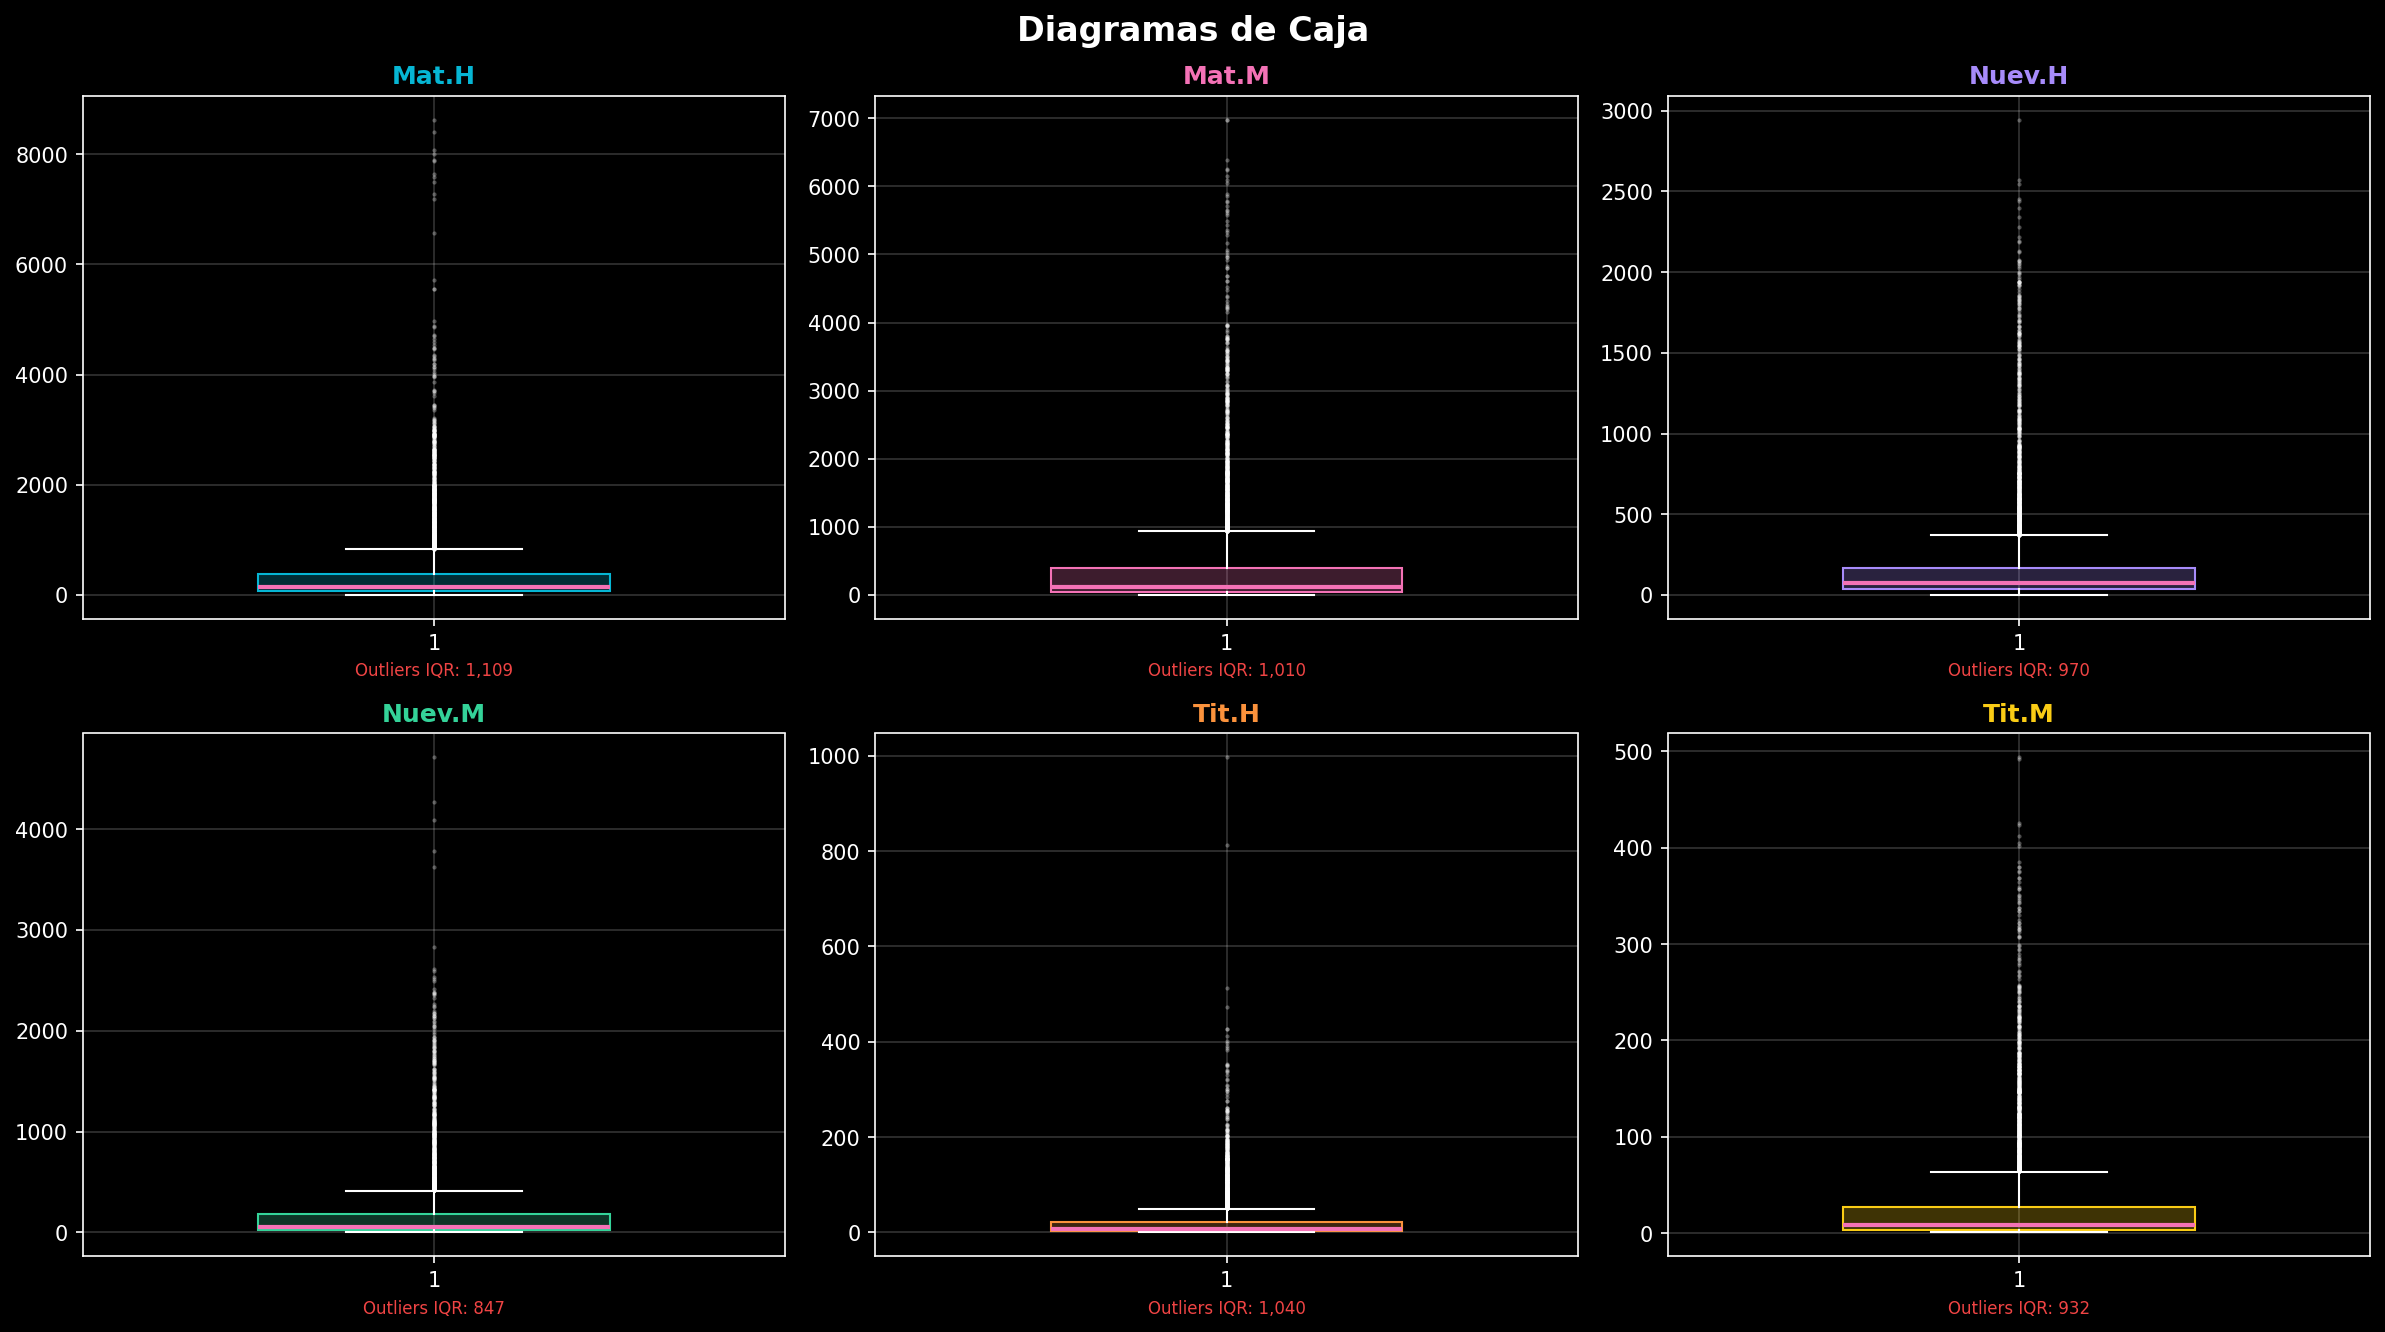
\includegraphics[width=0.8\textwidth]{fig1_boxplots.png} 
    \caption{Boxplot de las columnas numéricas}
    \label{fig:fig1}
\end{figure}

\begin{figure}[H]
    \centering
    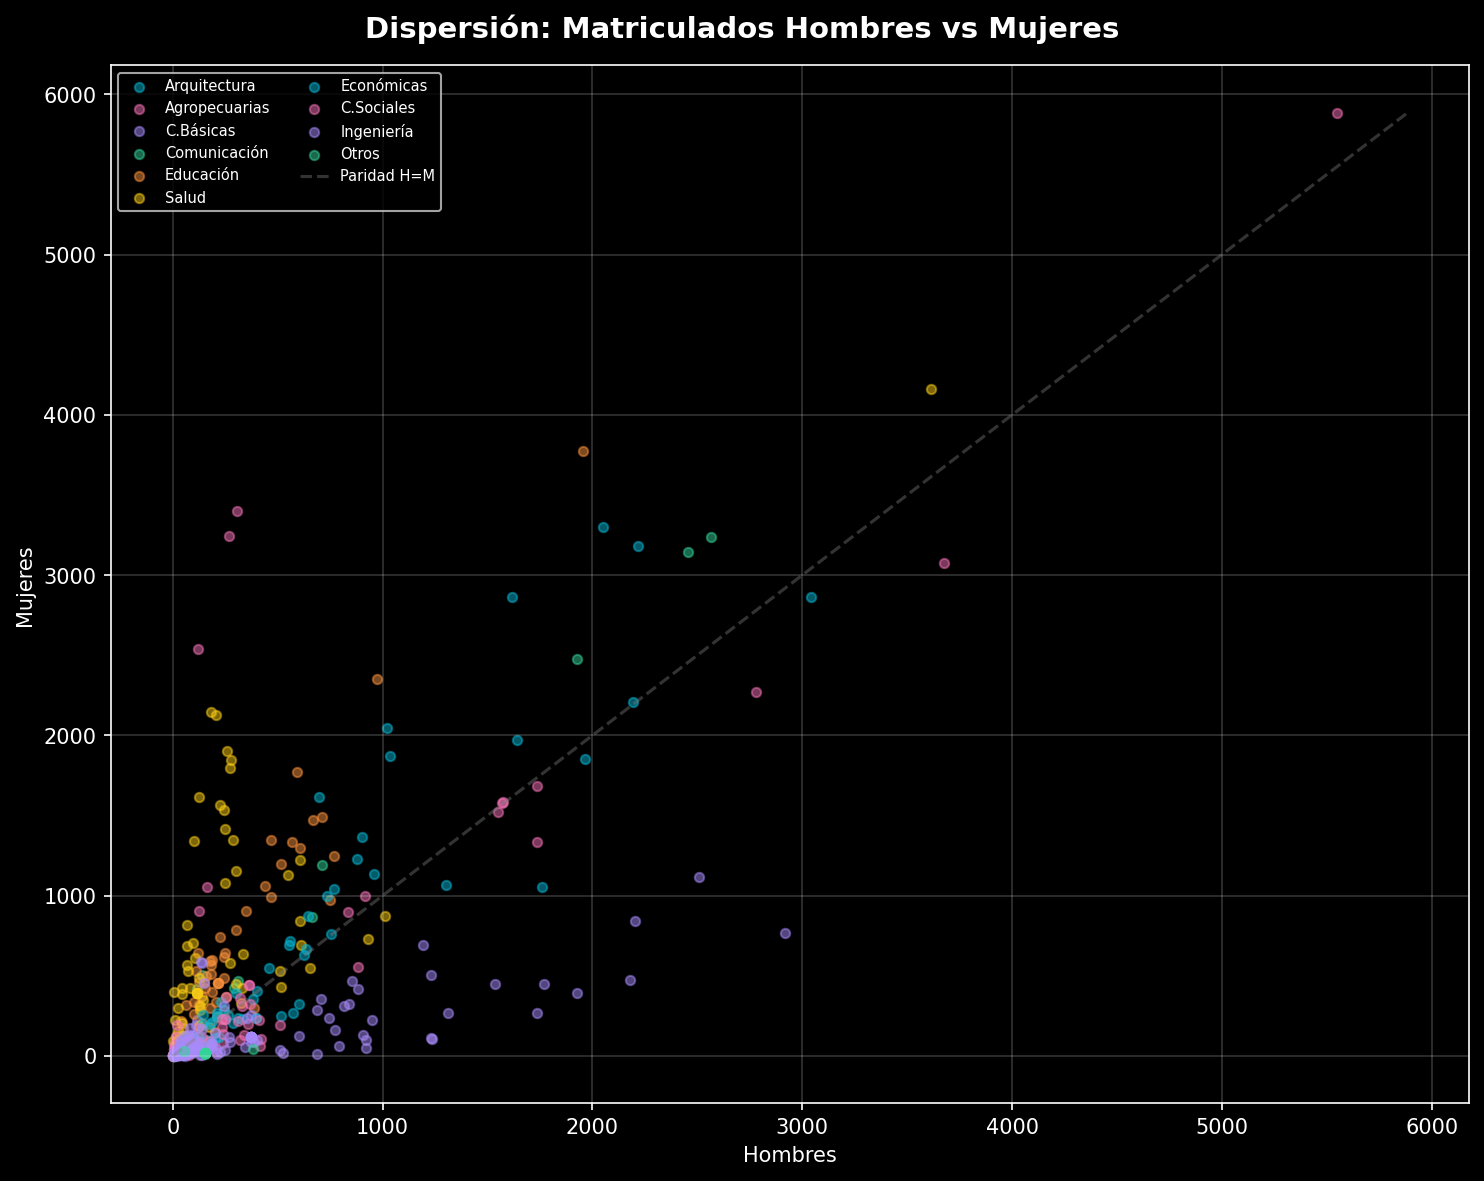
\includegraphics[width=0.8\textwidth]{fig2_dispersion.png} 
    \caption{Gráfico de dispersión}
    \label{fig:fig2}
\end{figure}

Esta difernecia entre los géneros y carreras se puede ver con mayor claridad en el gráfico \ref{fig:fig3}. Allí se puede ver como Salud efectivamente tiene la diferencia más marcada. Del mismo modo, las diferencias entre los departamentos se pueden ver en la figura \ref{fig:fig4}.

\begin{figure}[H]
    \centering
    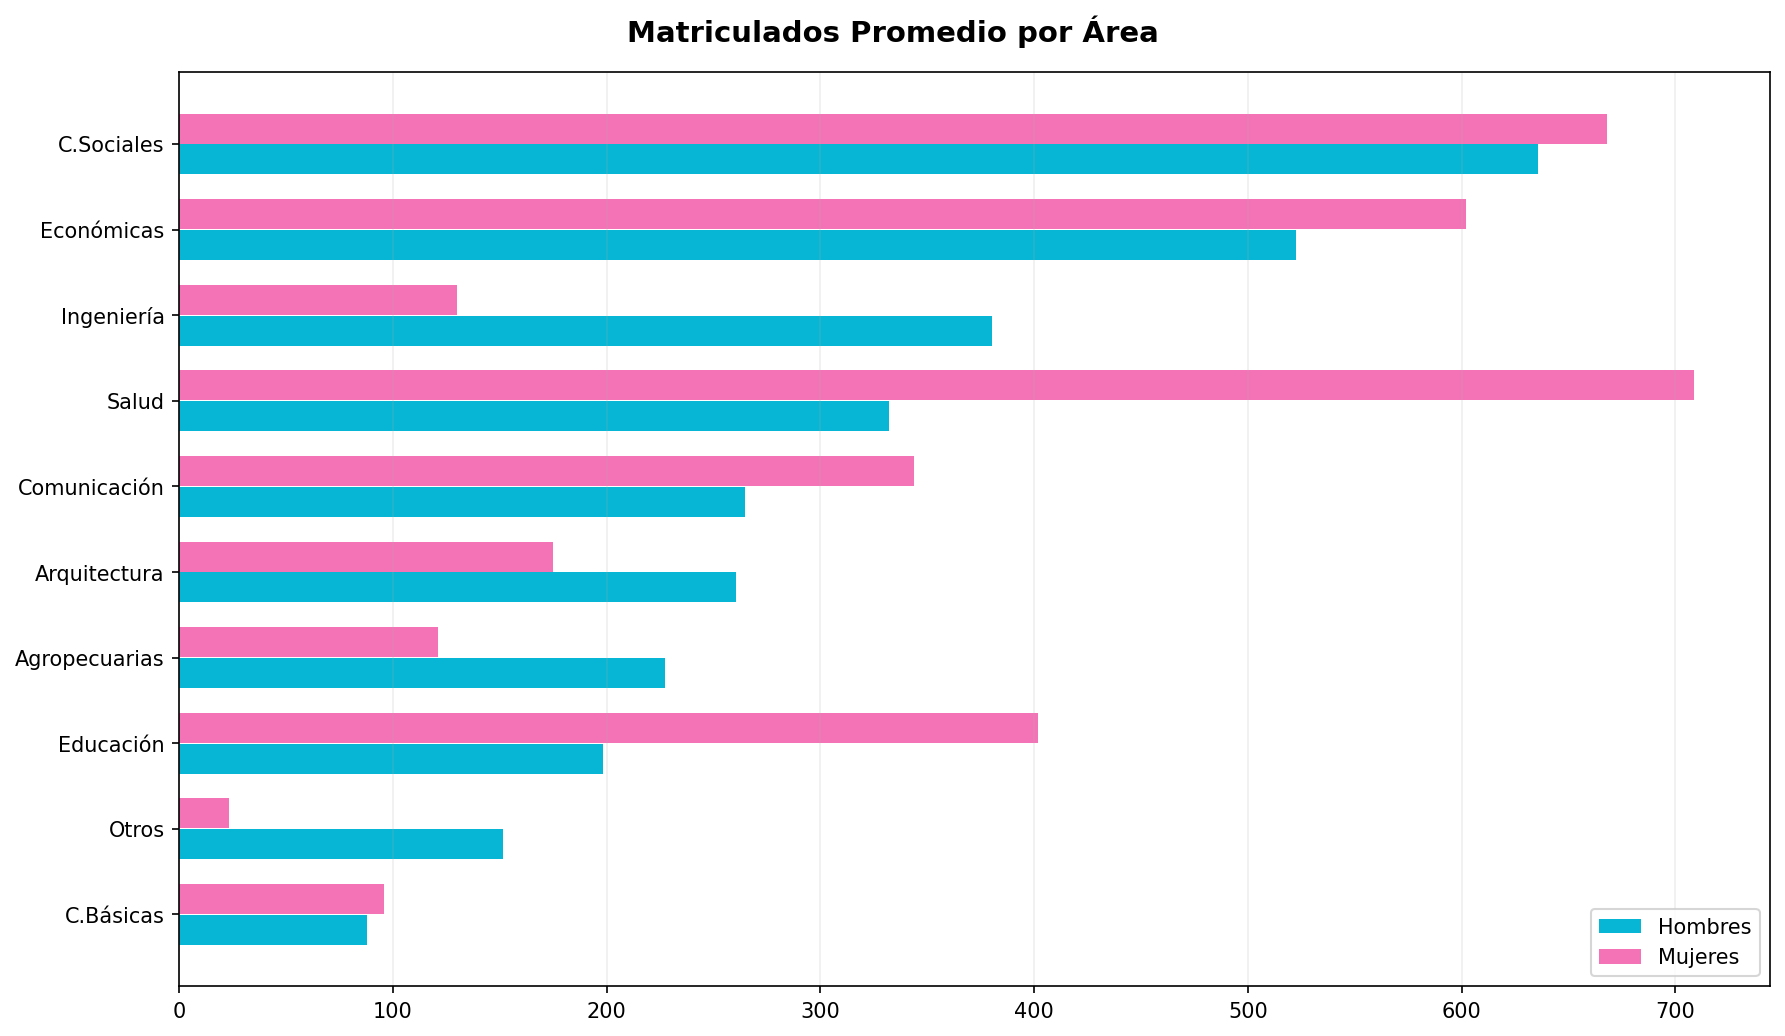
\includegraphics[width=0.8\textwidth]{fig3_barras_area.png} 
    \caption{Gráfico de barras por área}
    \label{fig:fig3}
\end{figure}

\begin{figure}[H]
    \centering
    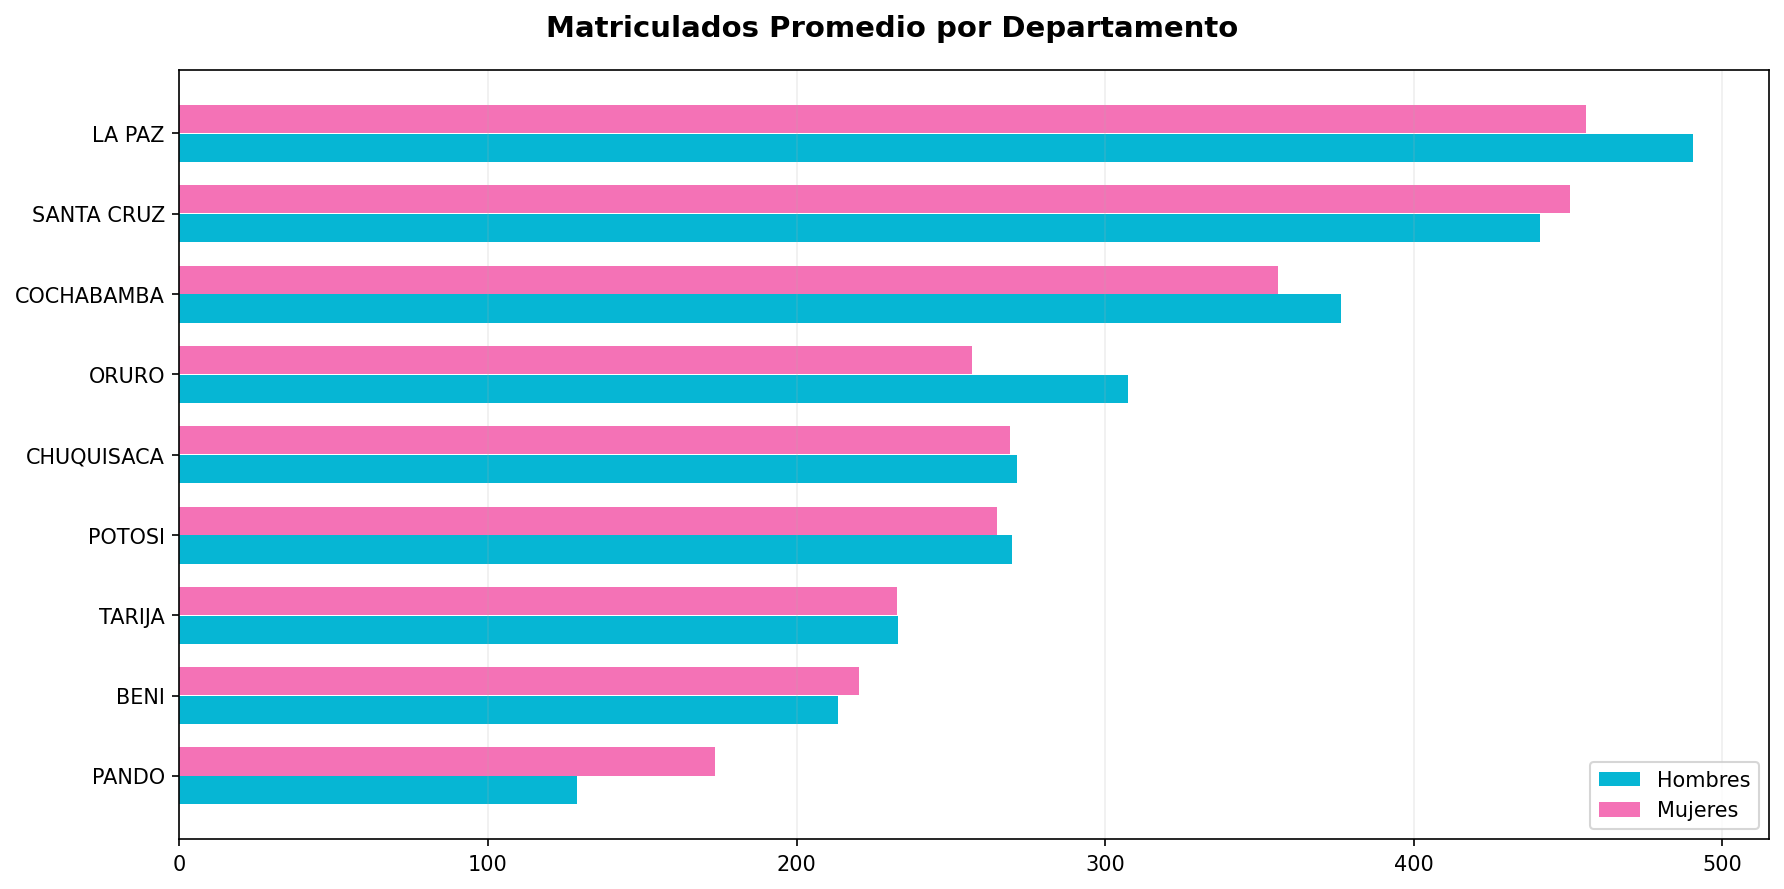
\includegraphics[width=0.8\textwidth]{fig4_barras_ciudad.png} 
    \caption{Gráfico de barras por ciudad}
    \label{fig:fig4}
\end{figure}

Como los datos tienen una columan para el tiempo, tambien podemos verlo en la \ref{fig:fig5} como una evolución temporal. Para ver como es que los datos están desbalanceados, se puede ver la \ref{fig:fig7}. En este caso la diferencia entre la mediana y la media es grande.

\begin{figure}[H]
    \centering
    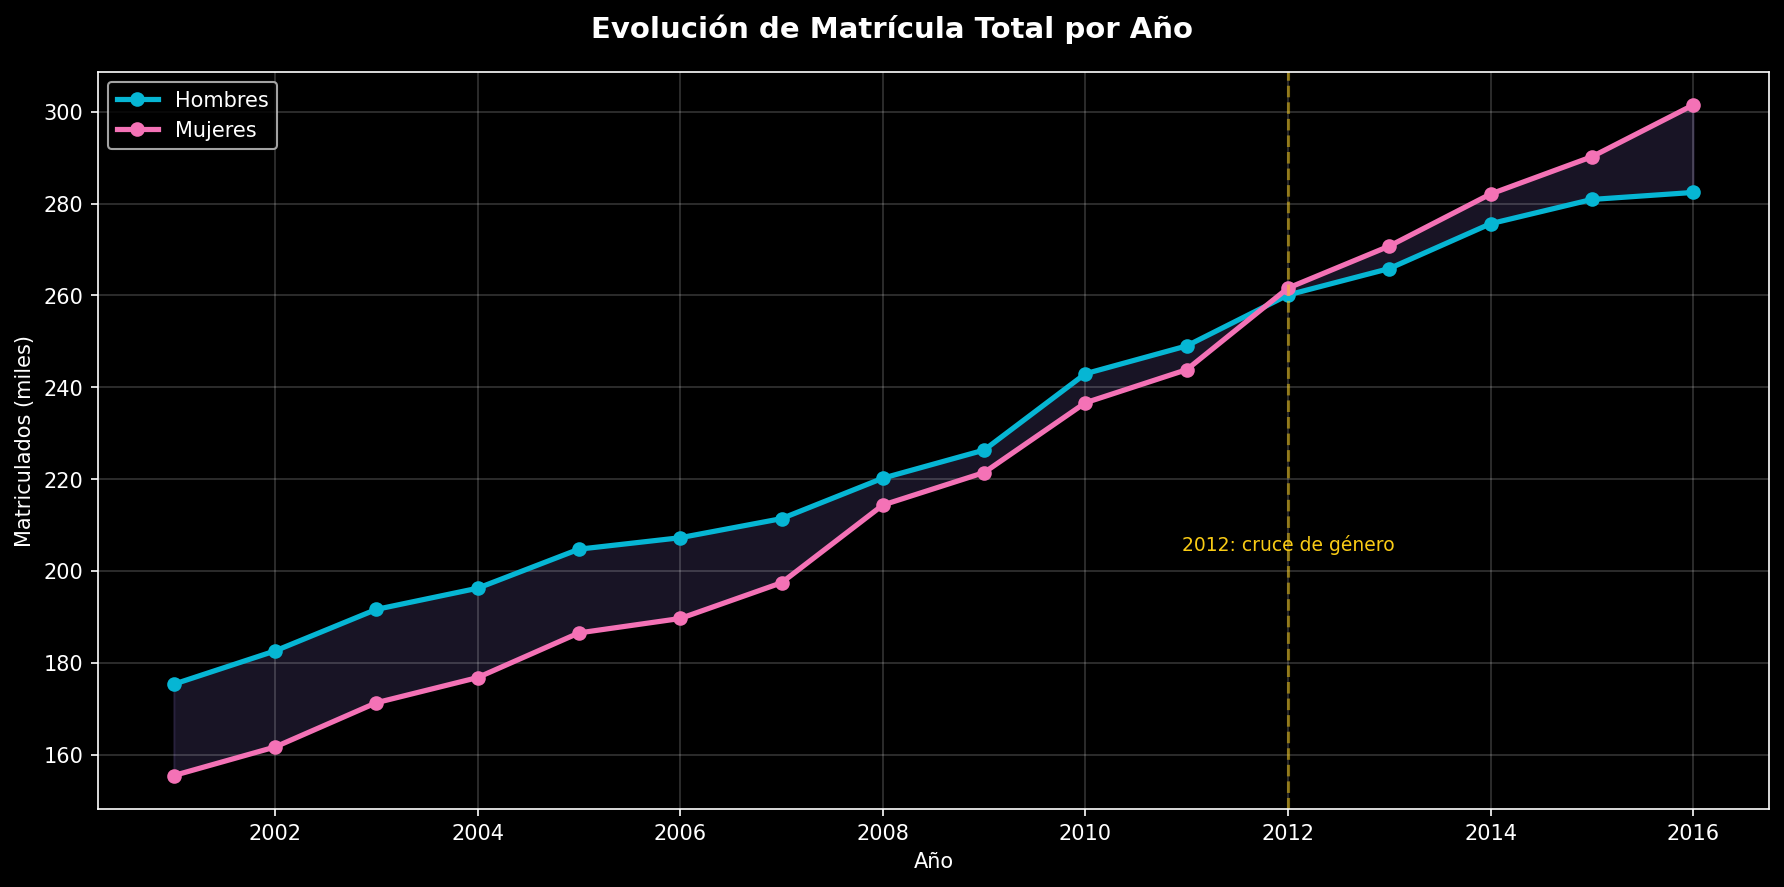
\includegraphics[width=0.8\textwidth]{fig5_evolucion.png} 
    \caption{Gráfico de barras por ciudad}
    \label{fig:fig5}
\end{figure}

\begin{figure}[H]
    \centering
    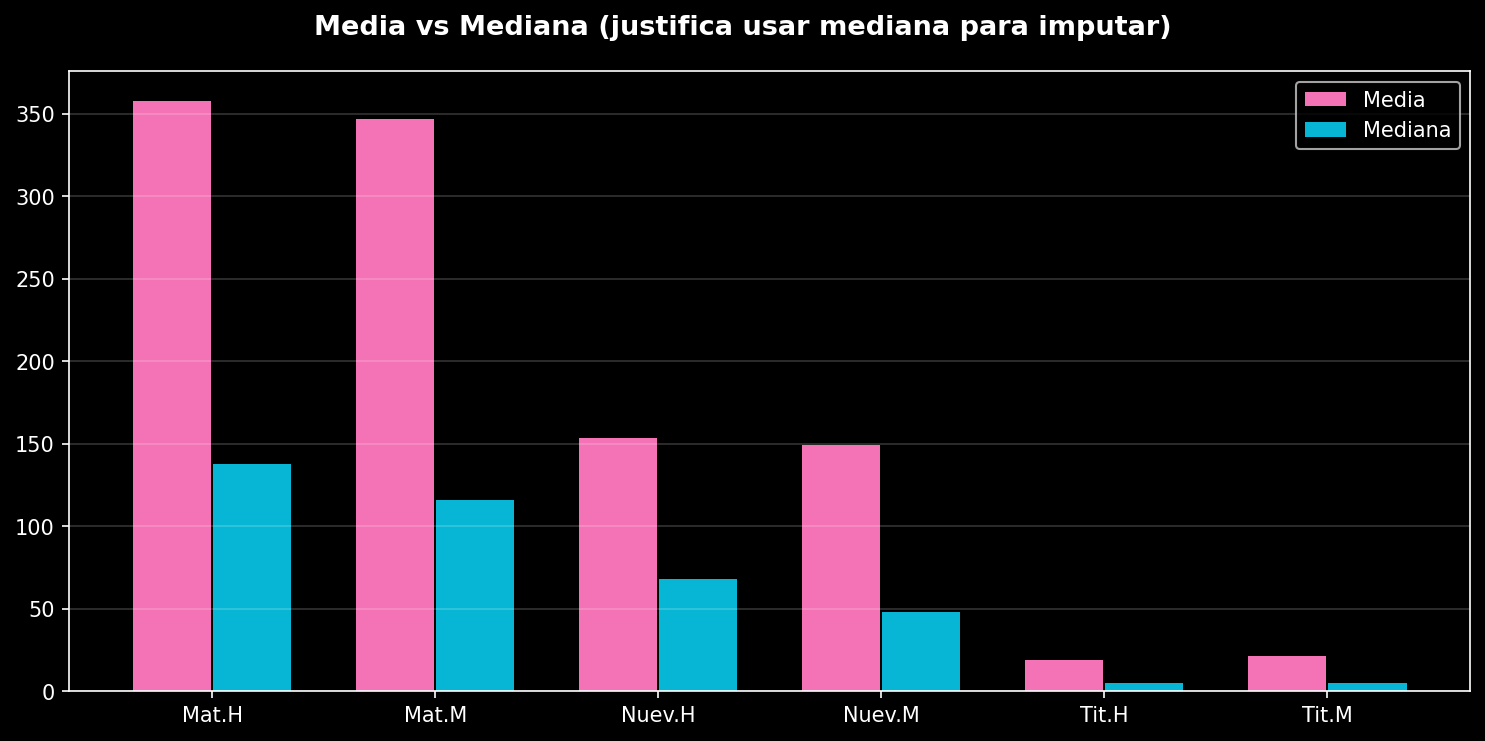
\includegraphics[width=0.8\textwidth]{fig7_media_vs_mediana.png} 
    \caption{Gráfico de barras por ciudad}
    \label{fig:fig7}
\end{figure}

Finalmente la comparación entre universidades públicas y privadas se puede ver en la \ref{fig:fig8}

\begin{figure}[H]
    \centering
    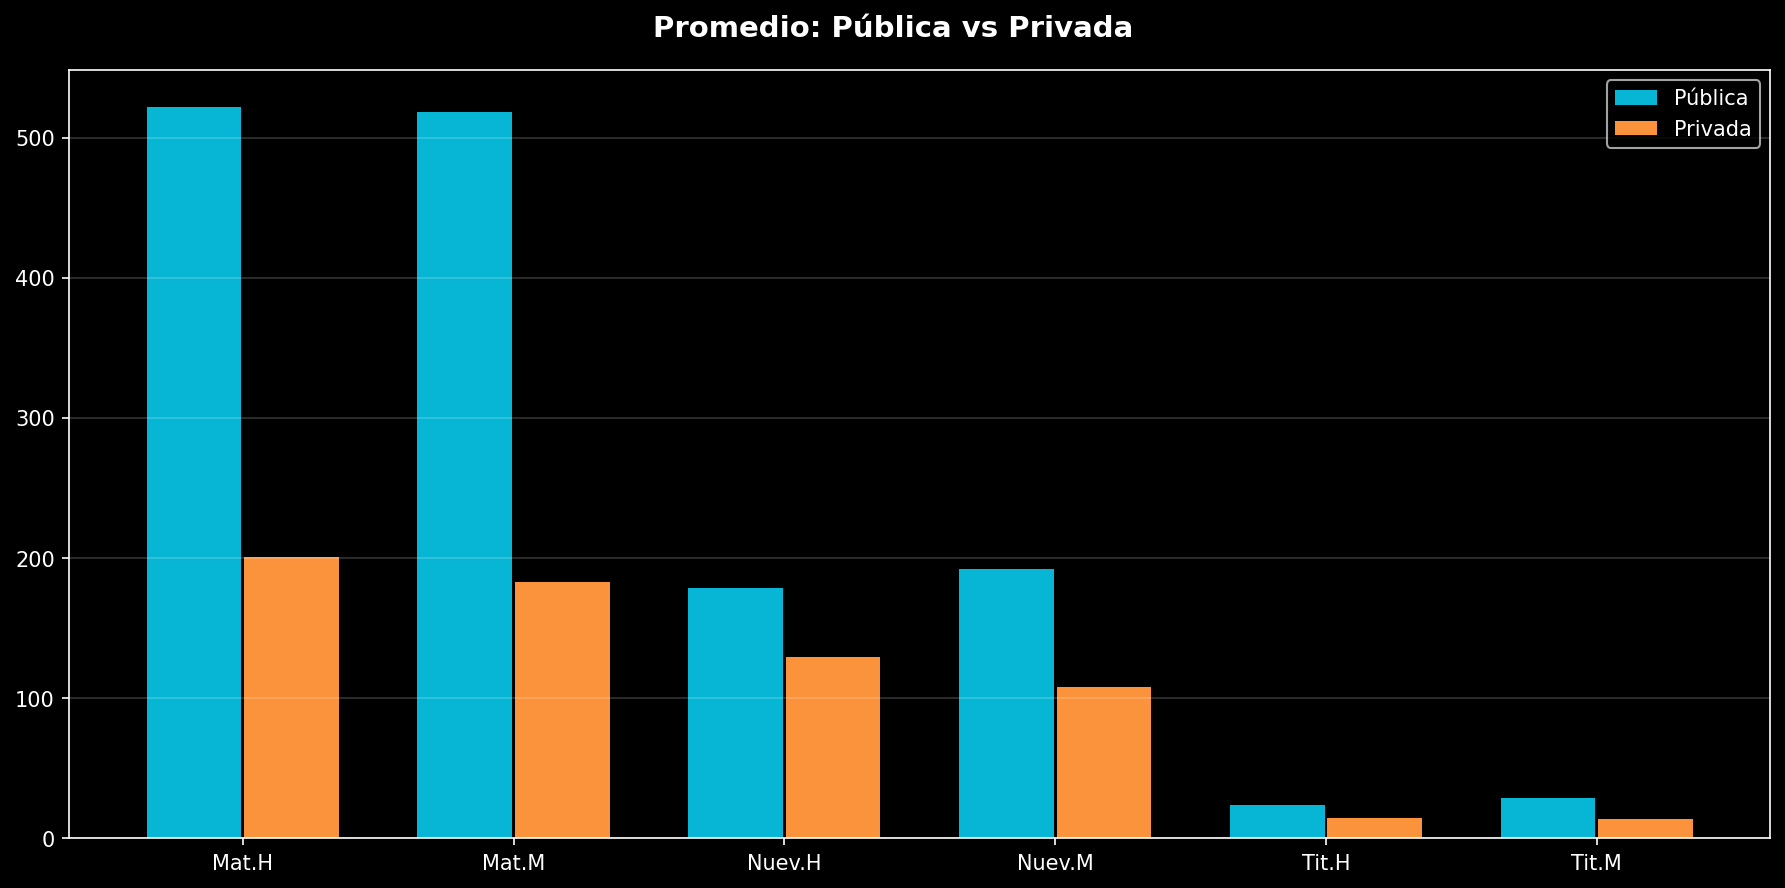
\includegraphics[width=0.8\textwidth]{fig8_publica_vs_privada.png} 
    \caption{Gráfico de barras por ciudad}
    \label{fig:fig8}
\end{figure}

También se usaron scripts de Python para sacar un resultado númerico:


\begin{verbatim}
============================================================
MÉTRICAS DESCRIPTIVAS
============================================================
   Var     N  Media  Mediana   Std  Mín    Máx  Asimetría  Curtosis
 Mat.H 10263  357.8    138.0 607.8  0.0 8628.0        4.7      35.5
 Mat.M 10263  347.0    116.0 633.0  0.0 6978.0        4.1      23.1
Nuev.H 10263  153.5     68.0 260.3  0.0 2944.0        4.1      22.0
Nuev.M 10263  149.2     48.0 283.8  0.0 4712.0        4.9      36.7
 Tit.H 10263   18.9      5.0  40.1  0.0  997.0        5.8      70.2
 Tit.M 10263   21.3      5.0  43.9  0.0  494.0        4.0      21.2
\end{verbatim}


\begin{verbatim}
============================================================
MÉTRICAS DESCRIPTIVAS
============================================================
                   Mat.H  Mat.M  Nuev.H  Nuev.M  Tit.H  Tit.M
TIPO DE EDUCACIÓN                                            
PRIVADA            200.7  183.1   129.6   108.3   14.4   13.8
PUBLICA            522.1  518.3   178.4   191.9   23.5   29.1
\end{verbatim}

\begin{verbatim}
============================================================
MÉTRICAS DESCRIPTIVAS
============================================================
            Hombres  Mujeres  Total
CIUDAD                             
LA PAZ        490.7    456.0  946.7
SANTA CRUZ    440.9    450.8  891.7
COCHABAMBA    376.5    356.1  732.6
ORURO         307.6    256.8  564.4
CHUQUISACA    271.4    269.2  540.6
POTOSI        270.0    265.1  535.1
TARIJA        233.0    232.6  465.6
BENI          213.3    220.4  433.7
PANDO         128.9    173.7  302.6
\end{verbatim}

\section*{Imputación de datos faltantes}

Para ver si existen datos faltantes se corrió un script que mostraba los mismos. El resultado fue este:

\begin{verbatim}
============================================================
2. DATOS FALTANTES
============================================================
  Filas sin datos (todos ceros): 2,301 (22.4%)

  Variable     Faltantes     Media   Mediana
  ------------ --------- --------- ---------
  Mat.H            2,301     417.3     176.0
  Mat.M            2,301     408.0     141.0
  Nuev.H           2,301     176.7      76.0
  Nuev.M           2,301     175.1      64.0
  Tit.H            2,301      21.3       6.0
  Tit.M            2,301      25.2       6.0

  Método: mediana por grupo (ÁREA + TIPO DE EDUCACIÓN)
  NaN restantes: 0
\end{verbatim}

Los datos fueron imputados con la mediana debido a que esta no incurre en un sesgo mayor como el que produce la media, que en este caso al ser una distribución sesgada podria producir un desbalance mayor.

\section*{Tratamiento de outliers}

Para detectar los outliers se utilizó dos métodos. El primero es el IQR en los cuartiles 1 y 3, con ello se puedo ver los siguiente:

\begin{verbatim}
============================================================
3. DETECCIÓN DE OUTLIERS
============================================================

   Método IQR (1.5 × IQR) 
  Var            Q1      Q3     IQR   Límite Outliers      %
  Mat.H          65     374     308      836    1,109  11.1%
  Mat.M          37     395     358      932    1,010  10.1%
  Nuev.H         36     170     134      371      970  10.1%
  Nuev.M         22     179     157      414      847   8.9%
  Tit.H           3      22      19       50    1,040  12.6%
  Tit.M           3      27      24       63      932  11.7%
\end{verbatim}

También se usó la Winsorización al 5 y 95\%

\begin{verbatim}
   Winsorización (P5 – P95) 
  Var          Media    → Win      Std    → Win   Afect
  Mat.H        366.7    322.4    612.6    407.0     991
  Mat.M        357.8    304.8    639.8    409.4     961
  Nuev.H       164.2    140.2    266.0    161.0     952
  Nuev.M       160.6    133.5    291.4    168.5     839
  Tit.H         23.4     20.3     43.5     29.0     411
  Tit.M         27.3     23.7     48.1     33.2     400
\end{verbatim}

Finalmente antes de realizar una acción se comparó ambos resultados:

\begin{verbatim}
   Comparativa 
  Var            IQR   Winsor
  Mat.H        1,109      991
  Mat.M        1,010      961
  Nuev.H         970      952
  Nuev.M         847      839
  Tit.H        1,040      411
  Tit.M          932      400
  → IQR es más estricto en todas las variables.
\end{verbatim}

Se escogió el segundo método ya que tenia muchos menos outliers y además los preservaba en vez de eliminarlos. Se puede ver un resultado gráfico en la \ref{fig:fig6}

\begin{figure}[H]
    \centering
    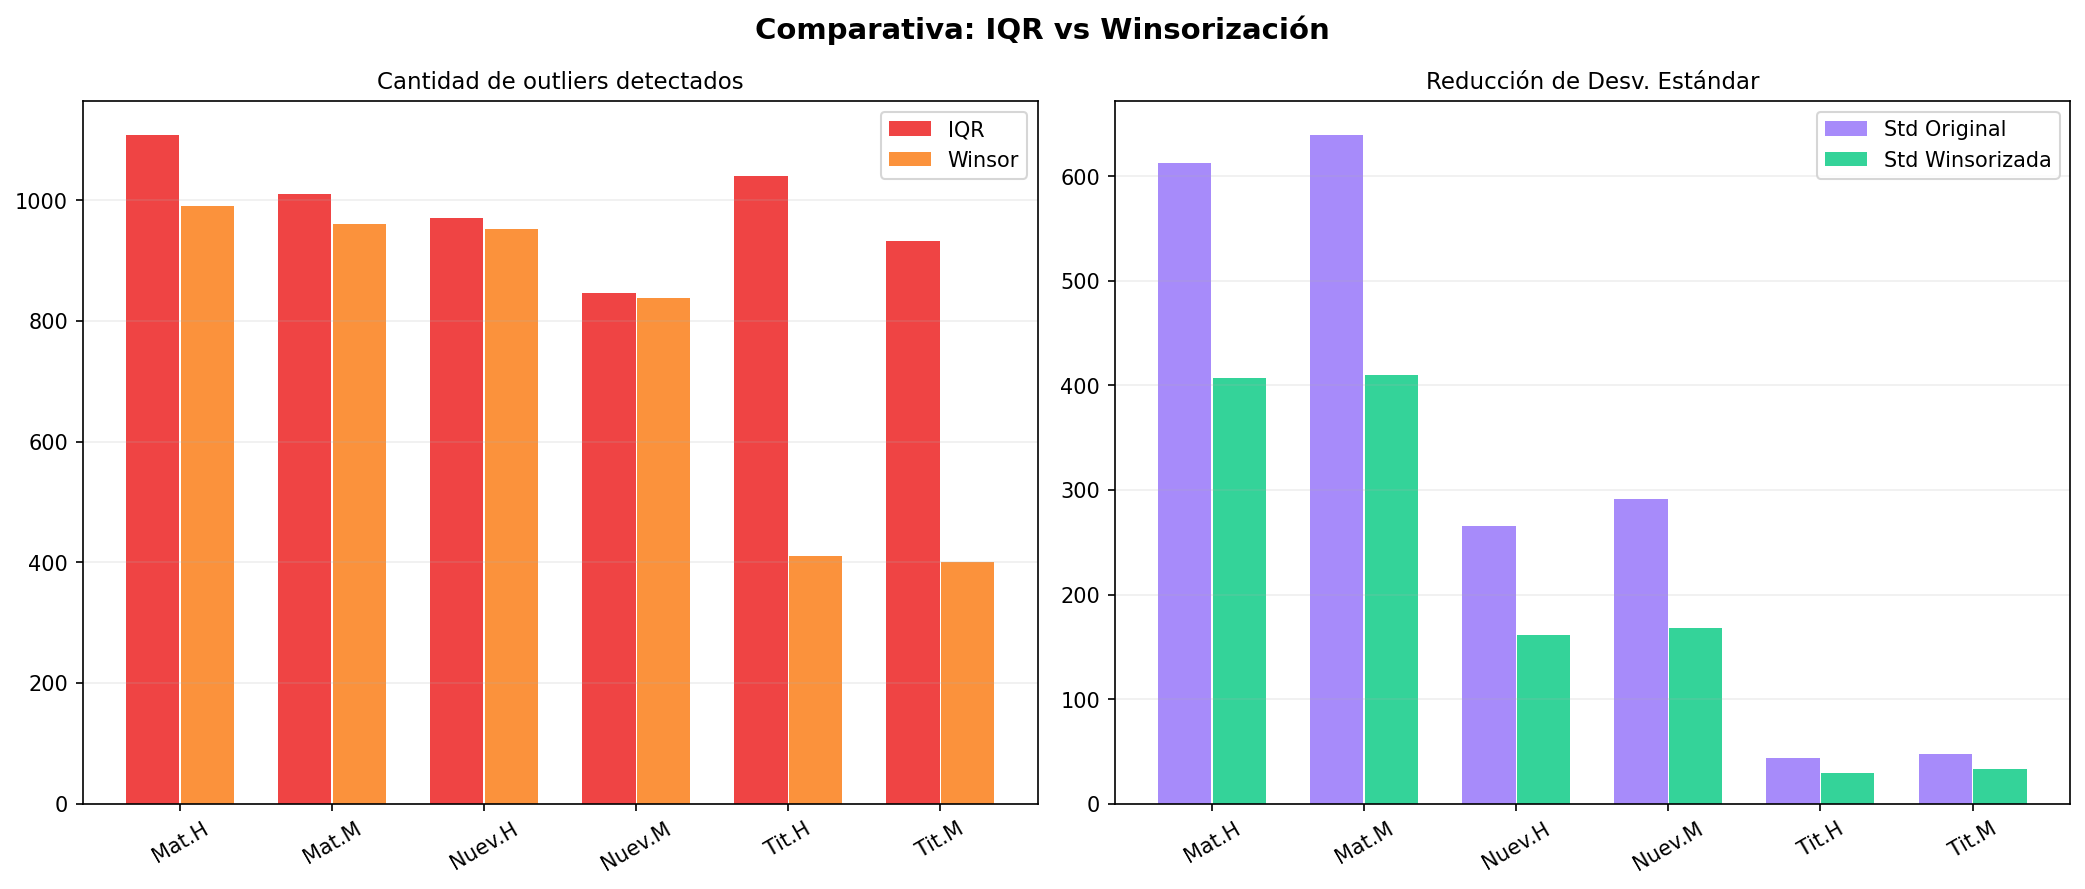
\includegraphics[width=0.8\textwidth]{fig6_comparativa_outliers.png} 
    \caption{Gráfico de barras por ciudad}
    \label{fig:fig6}
\end{figure}

\end{document}
